\documentclass[tikz,border=0pt]{standalone}
\usepackage{fontspec}
\hyphenpenalty=10000
\exhyphenpenalty=10000
\setmainfont[Path=../fonts/,BoldFont=Poppins-SemiBold.ttf,ItalicFont=Poppins-Italic.ttf]{Poppins-Regular.ttf}
\usepackage{pgfplots}
\pgfplotsset{compat=1.18}
\usetikzlibrary{calc,arrows.meta}
\definecolor{ink}{HTML}{161b22}
\definecolor{text}{HTML}{353535}
\definecolor{muted}{HTML}{646c74}
\definecolor{line}{HTML}{d7dadd}
\definecolor{wash}{HTML}{f6f6f6}
\definecolor{tint}{HTML}{e6ecef}
\definecolor{link}{HTML}{1d63b7}
\definecolor{local}{HTML}{376c97}
\definecolor{api}{HTML}{995d46}
\definecolor{cloud}{HTML}{7b649b}
\definecolor{match}{HTML}{7d9fc4}
\definecolor{miss}{HTML}{e0e3e5}
\definecolor{group}{HTML}{DCE2E5}
\definecolor{operation}{HTML}{C5CFD5}
\definecolor{mint}{HTML}{C9EEDF}
\definecolor{blueplane}{HTML}{AEC8E0}
\definecolor{pinkplane}{HTML}{F6D5DE}
\definecolor{peachplane}{HTML}{FFDBB8}
\definecolor{purpleplane}{HTML}{DCC7E7}
\begin{document}
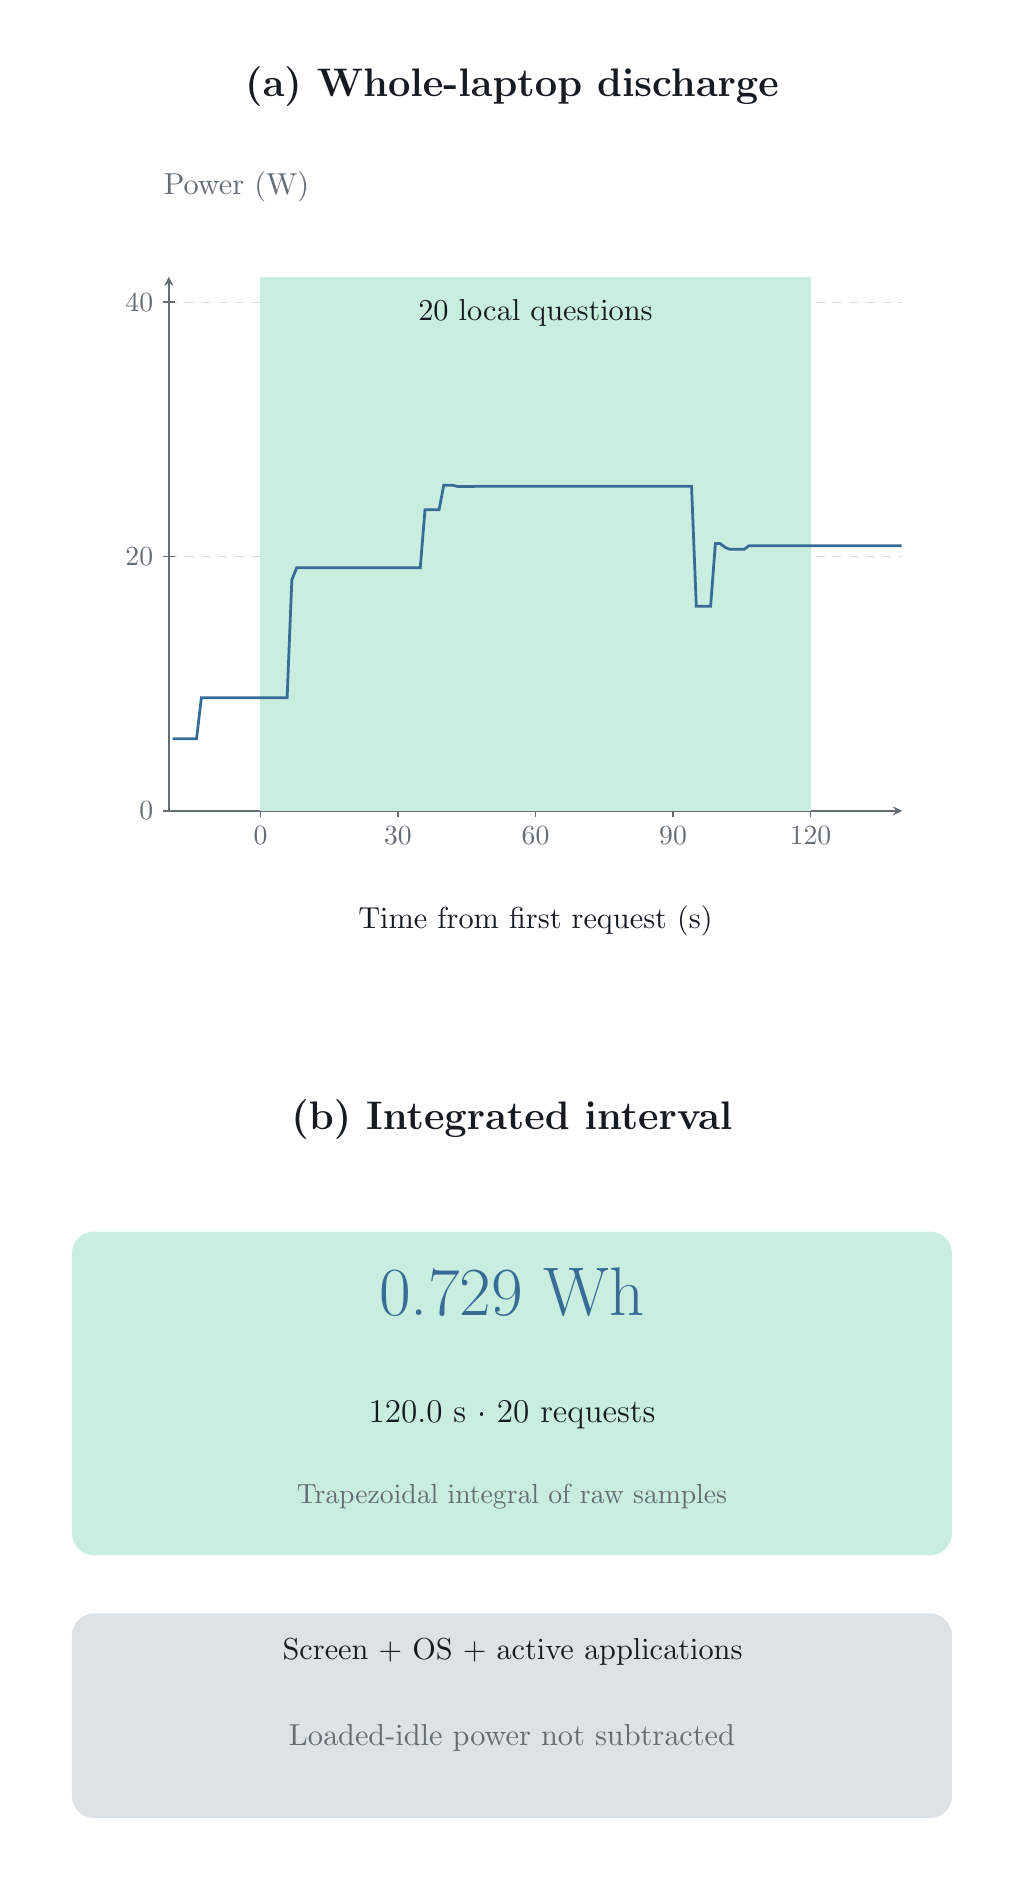
\begin{tikzpicture}[x=1pt,y=-1pt]
\path[use as bounding box] (0,0) rectangle (350,665);
\node[anchor=north west,inner sep=0pt,text=ink,align=center,font=\fontsize{14}{21.0}\selectfont,anchor=north] at (175.0,14) {\textbf{(a) Whole-laptop discharge}};
\node[anchor=north west,inner sep=0pt,text=muted,align=left,font=\fontsize{11}{16.5}\selectfont] at (49,52) {Power (W)};
\begin{axis}[at={(51pt,-90pt)},anchor=north west,width=265pt,height=193pt,scale only axis,
axis lines=left,axis line style={line width=.5pt,draw=muted},
tick style={line width=.5pt,draw=muted},tick label style={font=\fontsize{10}{15}\selectfont,text=muted},
xticklabel={\pgfmathprintnumber[assume math mode=true]{\tick}},
yticklabel={\pgfmathprintnumber[assume math mode=true]{\tick}},
ymajorgrids=true,grid style={line width=.3pt,draw=line,dashed},
xmin=-20,xmax=139.99300003051758,ymin=0,ymax=42,xtick={0,30,60,90,120},ytick={0,20,40},clip=true]
\path[fill=mint] (axis cs:0,0) rectangle (axis cs:119.99300003051758,42);
\node[anchor=north,font=\fontsize{10.5}{15}\selectfont,text=ink] at (axis cs:59.99650001525879,41) {20 local questions};
\addplot[local,line width=1pt,no marks] coordinates {(-19.178000,5.669000) (-18.090000,5.669000) (-17.047000,5.669000) (-16.025000,5.669000) (-14.987000,5.669000) (-13.947000,5.669000) (-12.897000,8.902000) (-11.853000,8.902000) (-10.819000,8.902000) (-9.775000,8.902000) (-8.738000,8.902000) (-7.685000,8.902000) (-6.645000,8.902000) (-5.603000,8.902000) (-4.562000,8.902000) (-3.521000,8.902000) (-2.453000,8.902000) (-1.408000,8.902000) (-0.377000,8.902000) (0.665000,8.902000) (1.685000,8.902000) (2.719000,8.902000) (3.749000,8.902000) (4.771000,8.902000) (5.812000,8.902000) (6.841000,18.169000) (7.884000,19.107000) (8.920000,19.107000) (9.945000,19.107000) (10.974000,19.107000) (12.003000,19.107000) (13.051000,19.107000) (14.098000,19.107000) (15.145000,19.107000) (16.186000,19.107000) (17.225000,19.107000) (18.285000,19.107000) (19.308000,19.107000) (20.355000,19.107000) (21.411000,19.107000) (22.449000,19.107000) (23.493000,19.107000) (24.519000,19.107000) (25.562000,19.107000) (26.585000,19.107000) (27.616000,19.107000) (28.666000,19.107000) (29.703000,19.107000) (30.734000,19.107000) (31.770000,19.107000) (32.796000,19.107000) (33.829000,19.107000) (34.855000,19.107000) (35.890000,23.674000) (36.905000,23.674000) (37.923000,23.674000) (38.958000,23.674000) (39.981000,25.600000) (41.014000,25.600000) (42.059000,25.600000) (43.081000,25.498000) (44.115000,25.498000) (45.145000,25.498000) (46.185000,25.498000) (47.232000,25.530000) (48.260000,25.530000) (49.293000,25.530000) (50.330000,25.530000) (51.353000,25.530000) (52.388000,25.530000) (53.424000,25.530000) (54.468000,25.530000) (55.501000,25.530000) (56.541000,25.530000) (57.582000,25.530000) (58.620000,25.530000) (59.660000,25.530000) (60.728000,25.530000) (61.761000,25.530000) (62.791000,25.530000) (63.821000,25.530000) (64.877000,25.530000) (65.909000,25.530000) (66.936000,25.530000) (67.965000,25.530000) (68.983000,25.530000) (70.016000,25.530000) (71.064000,25.530000) (72.116000,25.530000) (73.166000,25.530000) (74.242000,25.530000) (75.299000,25.530000) (76.342000,25.530000) (77.378000,25.530000) (78.411000,25.530000) (79.451000,25.530000) (80.491000,25.530000) (81.523000,25.530000) (82.562000,25.530000) (83.615000,25.530000) (84.656000,25.530000) (85.715000,25.530000) (86.763000,25.530000) (87.798000,25.530000) (88.828000,25.530000) (89.871000,25.530000) (90.912000,25.530000) (91.965000,25.530000) (92.993000,25.530000) (94.038000,25.530000) (95.079000,16.095000) (96.128000,16.095000) (97.165000,16.095000) (98.200000,16.095000) (99.242000,21.015000) (100.278000,21.015000) (101.342000,20.720000) (102.382000,20.567000) (103.423000,20.567000) (104.477000,20.567000) (105.518000,20.567000) (106.559000,20.840000) (107.602000,20.840000) (108.647000,20.840000) (109.707000,20.840000) (110.768000,20.840000) (111.835000,20.840000) (112.877000,20.840000) (113.910000,20.840000) (114.975000,20.840000) (116.024000,20.840000) (117.092000,20.840000) (118.140000,20.840000) (119.182000,20.840000) (120.230000,20.840000) (121.278000,20.840000) (122.351000,20.840000) (123.384000,20.840000) (124.415000,20.840000) (125.454000,20.840000) (126.490000,20.840000) (127.530000,20.840000) (128.550000,20.840000) (129.591000,20.840000) (130.607000,20.840000) (131.621000,20.840000) (132.645000,20.840000) (133.666000,20.840000) (134.697000,20.840000) (135.734000,20.840000) (136.777000,20.840000) (137.806000,20.840000) (138.829000,20.840000) (139.856000,20.840000)};
\end{axis}
\node[anchor=north west,inner sep=0pt,text=ink,align=center,font=\fontsize{11}{16.5}\selectfont,anchor=north] at (183.5,317) {Time from first request (s)};
\node[anchor=north west,inner sep=0pt,text=ink,align=center,font=\fontsize{14}{21.0}\selectfont,anchor=north] at (175.0,387) {\textbf{(b) Integrated interval}};
\path[fill=mint,rounded corners=8pt] (16,435) rectangle (334,552);
\node[anchor=north west,inner sep=0pt,text=local,align=center,font=\fontsize{28}{42.0}\selectfont,anchor=north] at (175.0,448) {0.729 Wh};
\node[anchor=north west,inner sep=0pt,text=ink,align=center,font=\fontsize{12}{18.0}\selectfont,anchor=north] at (175.0,496) {120.0 s · 20 requests};
\node[anchor=north west,inner sep=0pt,text=muted,align=center,font=\fontsize{10}{15.0}\selectfont,anchor=north] at (175.0,526) {Trapezoidal integral of raw samples};
\path[fill=group,rounded corners=8pt] (16,573) rectangle (334,647);
\node[anchor=north west,inner sep=0pt,text=ink,align=center,font=\fontsize{11}{16.5}\selectfont,text width=298pt] at (26.0,582) {Screen + OS + active applications};
\node[anchor=north west,inner sep=0pt,text=muted,align=center,font=\fontsize{10.5}{15.75}\selectfont,anchor=north] at (175.0,613) {Loaded-idle power not subtracted};

\end{tikzpicture}
\end{document}
